\documentclass{beamer}
\usepackage{../tut-slides}
\usepackage{../mathoperatorsAuD}

\usepackage{lmodern}
\usepackage{amsmath,amssymb}
\usepackage{wasysym}
\usepackage{stmaryrd}
\usepackage{enumerate}
%\usepackage[inline]{enumitem} 		%customize label
%\newcommand{\labelitemi}{\raisebox{1pt}{\scalebox{.9}{$\blacktriangleright$}}}
%\newcommand{\labelitemii}{$\vartriangleright$}
%\newcommand{\labelitemiii}{--}
\setbeamertemplate{itemize item}{\raisebox{1pt}{\scalebox{.9}{$\blacktriangleright$}}}
\setbeamertemplate{itemize subitem}{$\vartriangleright$}

\usepackage{booktabs}
\usepackage{tabularx}
\usepackage{tabu}
\newcommand*\head{\rowfont{\bfseries}}
\newcommand*{\tw}{\rowfont{\ttfamily}}
\renewcommand{\tabularxcolumn}[1]{>{\hspace{0pt}}m{#1}}
\usepackage{multirow}

\usepackage{cancel}

\usepackage{empheq}
\newcommand*\widefbox[1]{\fbox{\hspace{2em} #1 \hspace{2em}}}

\usepackage{tcolorbox}
\newtcolorbox{mymathbox}[1][]{colback=white, sharp corners, #1}

\usepackage{xcolor}
\usepackage{MnSymbol}

\newcommand{\col}[1]{\textcolor{cdpurple}{#1}}
\newcolumntype{R}[1]{>{\centering\arraybackslash}p{#1}}
\usepackage{tabularx}
\renewcommand{\tabularxcolumn}[1]{m{#1}}

\usepackage{qtree}
\usepackage[edges]{forest}

\DeclareMathOperator{\true}{true}
\DeclareMathOperator{\false}{false}


\begin{document}	
	\title{Algorithmen und Datenstrukturen}
	\subtitle{Übung 12: Aho-Hopcraft-Ullmann-Algorithmus}
	\author{Eric Kunze}
	\email{eric.kunze@mailbox.tu-dresden.de}
	\city{TU Dresden}
%	\institute{Lehrstuhl für Grundlagen der Programmierung}
	\titlegraphic{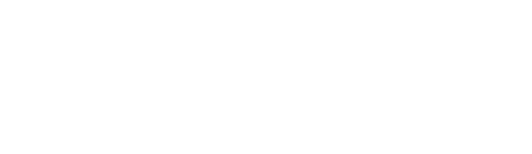
\includegraphics[width=2cm]{../TUD-white.pdf}}
	\date{29.01.2021}

	\maketitle

%%%%%%%%%%%%%%%%%%%%%%%%%%%%%%%%%%%%%%%%%%%%%%%%%%%%%%%%%%%%%%%%%%%%%%%%%%%%%%%%%%%

\section{Algebraisches Pfadproblem}

\begin{frame} \frametitle{Floyd-Warshall-Algorithmus}
	\small
	\begin{itemize}
		\item \textbf{Ziel}: kürzeste Wege in Graphem $G=(V,E,c)$
		\item $P^{(k)}_{u,v} =$ Menge aller Wege von $u$ nach $v$, deren innere Knoten in $\menge{1, \dots, k}$ liegen
		\item $D_G^{(k)} (u,v) = \begin{cases}
			\min\menge{c_p : p \in P_{u,v}^{(k)}} & \text{wenn } P_{u,v}^{(k)} \neq \emptyset \\
			\infty & \text{sonst}
		\end{cases}$
	
		\bigskip
		
		\item \textbf{Initialisierung}: $D_G^{(0)} = mA_G = \min\menge{A_G, \mathbf{0}_n} = \begin{cases}
		c(u,v) & \text{wenn } u \neq v, (u,v) \in E \\
		0 & \text{wenn } u = v \\
		\infty & \text{sonst}
		\end{cases}$
		\item \textbf{Rekursion}:
		\begin{equation*}
			\small
			\setlength{\arraycolsep}{1pt}
			\begin{array}{rclcccccl}
				D_G^{(k+1)}(u,v) &=& \min \Big\{ & D_G^{(k)}(u,v) & , & D_G^{(k)}(u,k+1) & + & D_G^{(k)}(k+1,v) & \Big\}  \\
				&=& \min \Big\{ & \text{alt} & , & \text{Zeile} & + & \text{Spalte} & \Big\}
			\end{array}
		\end{equation*}
	\end{itemize}
\end{frame}

\begin{frame} \frametitle{Abstraktion: algebraisches Pfadproblem}
	\small
	\begin{itemize}
		\item \textbf{bisher:} kürzeste Wege
		\begin{itemize}
			\item Summation $+$ entlang der Pfade
			\item Minimum $\min$ über alle Pfade
		\end{itemize}
		\item \textbf{jetzt:} Verallgemeinerung
		\begin{itemize}
			\item Pfadoperation $\odot$ entlang der Pfade
			\item Akkumulationsoperation $\oplus$
		\end{itemize}
		\item \textbf{Ergebnis:} allgemeine algebraische Struktur --- Semiring $(S, \oplus, \odot, \mathbf{0}, \mathbf{1})$
	\end{itemize}

	\centering
	
	\begin{tabular}{lccccc}
		\hline
		& Werte $S$ & $\oplus$ & $\odot$ & $\mathbf{0}$ & $\mathbf{1}$ \\
		\hline
		kürzeste Wegeproblem & $\R_{\ge 0}^\infty$ & $\min$ & $+$ & $\infty$ & $0$ \\
		Kapazitätsproblem & $\N_\infty$ & $\max$ & $\min$ & $0$ & $\infty$ \\
		Erreichbarkeitsproblem & $\menge{\true, \false}$ & $\lor$ & $\land$ & $\false$ & $\true$ \\
		Zuverlässigkeitsproblem & $[0,1]$ & $\max$ & $\cdot$ & $0$ & $1$ \\
		Prozessproblem & $\mathcal{P}(\Sigma^\ast)$ & $\cup$ & $\circ$ & $\emptyset$ & $\menge{\epsilon}$ \\ \hline
	\end{tabular}
\end{frame}

\begin{frame} \frametitle{Floyd-Warshall $\to$ Aho-Hopcraft-Ullmann}
	\begin{itemize}
		\item modifizierte Adjazenzmatrix $mA_G = \begin{cases}
		A_G(u,v) & \text{wenn } u \neq v \\
		A_G(u,v) \oplus \mathbf{1} & \text{wenn } u = v
		\end{cases}$
		\item \textbf{Initialisierung}: $D_G^{(0)} = mA_G$
		\item \textbf{Rekursion}:
		\begin{equation*} \small
		\boxed{\begin{aligned}
			&D_G^{(k+1)}(u,v) \\
			= \enskip &D_G^{(k)}(u,v) \textcolor{cdorange}{\oplus} \brackets{D_G^{(k)}(u,k+1) \textcolor{cdpurple}{\odot} (D_G^{(k)}(k+1,k+1))^\ast \textcolor{cdpurple}{\odot} D_G^{(k)}(k+1,v)}
			\end{aligned}}
		\end{equation*}
		\color{cdgray}
		\item vgl. dazu Floyd-Warshall:
		\begin{equation*}
			\begin{aligned}
				&D_G^{(k+1)}(u,v) \\
				= \enskip &\textcolor{cdorange}{\min}\menge{D_G^{(k)}(u,v) , D_G^{(k)}(u,k+1) \textcolor{cdpurple}{\boldsymbol{+}}
				0
				\textcolor{cdpurple}{\boldsymbol{+}}
				D_G^{(k)}(k+1,v)}
			\end{aligned}
			\end{equation*}
	\end{itemize}
\end{frame}

%%%%%%%%%%%%%%%%%%%%%%%%%%%%%%%%%%%%%%%%%%%%%%%%%%%%%%%%%%%%%%%%%%%%%%%%%%%%%%%%%%%

\begin{frame} \frametitle{Aufgabe 1}
	\begin{minipage}{\dimexpr0.4\linewidth-\fboxrule-\fboxsep}
		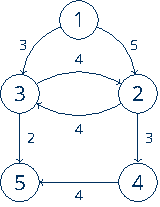
\includegraphics[width=\linewidth]{./tut12_task1-graph.pdf}
	\end{minipage}
	\pause
	\begin{minipage}{\dimexpr0.6\linewidth-\fboxrule-\fboxsep}
		\centering
		\textbf{Teil (a)} : \\
		$(S, \oplus, \odot, \mathbf{0}, \mathbf{1}) = (\N_\infty, \max, \min, 0, \infty)$
		
		\hspace{1em} \pause
		
		\textbf{Teil (b)} : \\
		$mA_G = D_G^{(0)} = \begin{pmatrix}
		\infty & 5      & 3      & 0      & 0 \\
		0      & \infty & 4      & 3      & 0 \\
		0      & 4      & \infty & 0      & 2 \\
		0      & 0      & 0      & \infty & 4 \\
		0      & 0      & 0      & 0      & \infty \\
		\end{pmatrix}$	
	\end{minipage}
\end{frame}

\begin{frame} \frametitle{Aufgabe 1}
	\textbf{Teil (c)} :
	\small
	Laut Vorlesung gilt $s^\ast = \sum_{n \in \N}^{\oplus} s^n$ mit $s^0 = \mathbf{1}$ und $s^{n+1} = s \odot s^n$. Im Semiring $(\N_\infty, \max, \min, 0, \infty)$ gilt:
	\begin{itemize}
		\item $s^0 = \mathbf{1} = \infty$
		\item $s^1 = s \odot s^0 = \min \menge{s, \infty} = s$
		\item $s^2 = s \odot s^1 = \min \menge{s, s} = s$
		\item ...
	\end{itemize}
	Schließlich ist $s^\ast = \sum_{n \in \N}^{\max} s^n = \sup \menge{s^n : n \in \N} = \sup \menge{\infty , s, s, \dots} = \infty = \mathbf{1}$.
	
	Somit gilt dann in der Updateformel 
	\begin{equation*}
	\begin{aligned}
		D_G^{(k+1)}(u,v) &= \max \menge{D_G^{(k)}(u,v) , \min\menge{D_G^{(k)}(u,k+1) , \infty, D_G^{(k)}(k+1,v)}} \\
		&=	\max \menge{D_G^{(k)}(u,v) , \min\menge{D_G^{(k)}(u,k+1), D_G^{(k)}(k+1,v)}} \\
		&= 	D_G^{(k)}(u,v) \oplus \brackets{D_G^{(k)}(u,k+1) \odot D_G^{(k)}(k+1,v)}
	\end{aligned}
	\end{equation*}
\end{frame}
\begin{frame} \frametitle{Aufgabe 1}
	\textbf{Teil (d)} :
	\begin{itemize}
		\item $D_G^{(1)}$: \hspace{.5em} keine Änderung (Quelle)
		\item $D_G^{(2)}$: \hspace{.5em} $(1,3,4)$, $(3,4,3)$, $(1,4,3)$
		\item $D_G^{(3)}$: \hspace{.5em} $(1,5,2)$, $(2,5,2)$
		\item $D_G^{(4)}$: \hspace{.5em} $(1,5,3)$, $(2,5,3)$, $(3,5,3)$
		\item $D_G^{(5)}$: \hspace{.5em} keine Änderung (Senke)
	\end{itemize}
	
	\pause
	
	\textbf{Teil (e)} :
	
	$D_{G'}(1,5) = 2$ über den Pfad $(1,2,3,5)$
\end{frame}


%%%%%%%%%%%%%%%%%%%%%%%%%%%%%%%%%%%%%%%%%%%%%%%%%%%%%%%%%%%%%%%%%%%%%%%%%%%%%%%%%%%


\begin{frame} \frametitle{Aufgabe 2}
	\begin{minipage}{\dimexpr0.5\linewidth-\fboxrule-\fboxsep}
		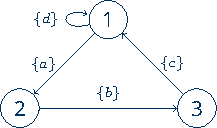
\includegraphics[width=\linewidth]{./tut12_task2-graph.pdf}
	\end{minipage} 
	\pause
	\begin{minipage}{\dimexpr0.5\linewidth-\fboxrule-\fboxsep}
		\centering
		\textbf{Teil (a)} : \\
		$(S, \oplus, \odot, \mathbf{0}, \mathbf{1}) = (\mathcal{P}(\Sigma^\ast), \cup, \circ, \emptyset, \menge{\epsilon})$
	\end{minipage}

	\hspace{1em} \pause
	
	Update-Formel: 
	\begin{equation*}
	\small
	\setlength{\arraycolsep}{1pt}
		\begin{array}{rccrcccccr}
			\mathrlap{D_G^{(k+1)}(u,v)}\\
			=& D_G^{(k)}(u,v) &\oplus& \Big( & D_G^{(k)}(u,k+1) &\odot& (D_G^{(k)}(k+1,k+1))^\ast &\odot& D_G^{(k)}(k+1,v) & \Big) \\
			=& D_G^{(k)}(u,v) &\cup& \Big( & D_G^{(k)}(u,k+1) &\circ& \alert{(D_G^{(k)}(k+1,k+1))^\ast} &\circ& D_G^{(k)}(k+1,v) & \Big) \\
			=& \text{alt} &\cup& \Big(& \text{Zeile} &\circ& \alert{(\text{Diagonale})^\ast} &\circ& \text{Spalte} & \Big)
		\end{array}
	\end{equation*}
\end{frame}

\begin{frame} \frametitle{Aufgabe 2}
	\textbf{Teil (b)} : \hspace{1em}
	$mA_G = D_G^{(0)} = \begin{pmatrix}
	\menge{\epsilon, d} & \menge{a} & \emptyset \\
	\emptyset & \menge{\epsilon} & \menge{b} \\
	\menge{c} & \emptyset & \menge{\epsilon} \\
	\end{pmatrix}$
	
	\pause
		
	\textbf{Teil (c)} :  \hspace{1em}
	$D_G^{(1)} = \begin{pmatrix}
	\menge{d}^\ast & \menge{d}^\ast \menge{a} & \emptyset \\
	\emptyset & \menge{\epsilon} & \menge{b} \\
	\menge{c}\menge{d}^\ast & \menge{c}\menge{d}^\ast \menge{a} & \menge{\epsilon} \\
	\end{pmatrix}$
\end{frame}


\begin{frame} \frametitle{Aufgabe 2}
	\textbf{Teil (d)} : 
	
	\small
	\begin{align*}
		D_G^{(2)}(3,3) 
		&= D_G^{(1)}(3,3) \cup \brackets{D_G^{(1)}(3,2) \circ (D_G^{(1)}(2,2))^\ast \circ D_G^{(1)}(2,3)} \\
		&= \menge{\epsilon} \cup \brackets{\menge{c} \menge{d}^\ast \menge{a} \circ \menge{\epsilon}^\ast \circ \menge{b}} \\
		&= \menge{\epsilon} \cup \brackets{\menge{c}\menge{d}^\ast \menge{ab}} \\
		~\\
		\onslide<2->{%
		D_G^{(3)}(3,3)
		&= D_G^{(2)}(3,3) \cup \brackets{D_G^{(2)}(3,3) \circ (D_G^{(2)}(3,3))^\ast \circ D_G^{(2)}(3,3)} \\
		&= D_G^{(2)}(3,3) \cup \brackets{D_G^{(2)}(3,3)}^\ast \\
		&= \brackets{D_G^{2}(3,3)}^\ast \\
		&= \brackets{\menge{\epsilon} \cup \menge{c}\menge{d}^\ast \menge{ab}}^\ast \\
		&= \brackets{\menge{c}\menge{d}^\ast \menge{ab}}^\ast }
	\end{align*}
\end{frame}
\end{document}
